% (c) 2002 Matthew Boedicker <mboedick@mboedick.org> (original author) http://mboedick.org
% (c) 2003-2007 David J. Grant <davidgrant-at-gmail.com> http://www.davidgrant.ca
% (c) 2008-2011 Nathaniel Johnston <nathaniel@nathanieljohnston.com> http://www.nathanieljohnston.com
%
%This work is licensed under the Creative Commons Attribution-Noncommercial-Share Alike 2.5 License. To view a copy of this license, visit http://creativecommons.org/licenses/by-nc-sa/2.5/ or send a letter to Creative Commons, 543 Howard Street, 5th Floor, San Francisco, California, 94105, USA.


\documentclass[letterpaper,11pt]{article} %%% 10
\usepackage[utf8]{inputenc}
\usepackage[french]{babel}
\newlength{\outerbordwidth}
\pagestyle{empty}
\raggedbottom
\raggedright
\usepackage[svgnames]{xcolor}
\usepackage{enumerate}
\usepackage{framed}
\usepackage{hyperref}
\usepackage{tocloft}
\usepackage{graphicx}
\usepackage{wrapfig}
%%\usepackage{fullpage}

%-----------------------------------------------------------
%Edit these values as you see fit

\setlength{\outerbordwidth}{3pt}  % Width of border outside of title bars
\definecolor{shadecolor}{gray}{0.75}  % Outer background color of title bars (0 = black, 1 = white)
\definecolor{shadecolorB}{gray}{0.93}  % Inner background color of title bars


%-----------------------------------------------------------
%Margin setup

\setlength{\evensidemargin}{-0.25in}
\setlength{\headheight}{0in}
\setlength{\headsep}{0in}
\setlength{\oddsidemargin}{-0.25in}
\setlength{\paperheight}{11in}
\setlength{\paperwidth}{8.5in}
\setlength{\tabcolsep}{0in}
\setlength{\textheight}{10.0in} %hauteur du text
\setlength{\textwidth}{7in}
\setlength{\topmargin}{-0.15in} %début de la marge en haut 
\setlength{\topskip}{0in}
\setlength{\voffset}{0.1in}


%-----------------------------------------------------------
%Custom commands
\newcommand{\resitem}[1]{\item[] #1 \vspace{2pt}}
\newcommand{\resheading}[1]{\vspace{2pt}
  \parbox{\textwidth}{\setlength{\FrameSep}{\fboxsep}
    \begin{shaded}
      \setlength{\fboxsep}{0pt}\framebox[\textwidth][l]{\setlength{\fboxsep}{4pt}\fcolorbox{shadecolorB}{shadecolorB}{\textbf{\sffamily{\mbox{~}\makebox[6.762in][l]{\large #1} \vphantom{p\^{E}}}}}}
    \end{shaded}
  }\vspace{-5pt}
}

\newcommand{\ressubheading}[4]{
  \begin{tabular*}{6.5in}{l@{\cftdotfill{\cftsecdotsep}\extracolsep{\fill}}r}
    \textbf{#1} & #2 \\
    \textit{#3} & \textit{#4} \\
  \end{tabular*}\vspace{-2pt}
}
%-----------------------------------------------------------

%\newcommand\ressourcepath{ressources/}

\begin{document}


%% \begin{wrapfigure}{R}{0.20\textwidth}
%%   \vspace{-65pt}
%%   \begin{center}
%%     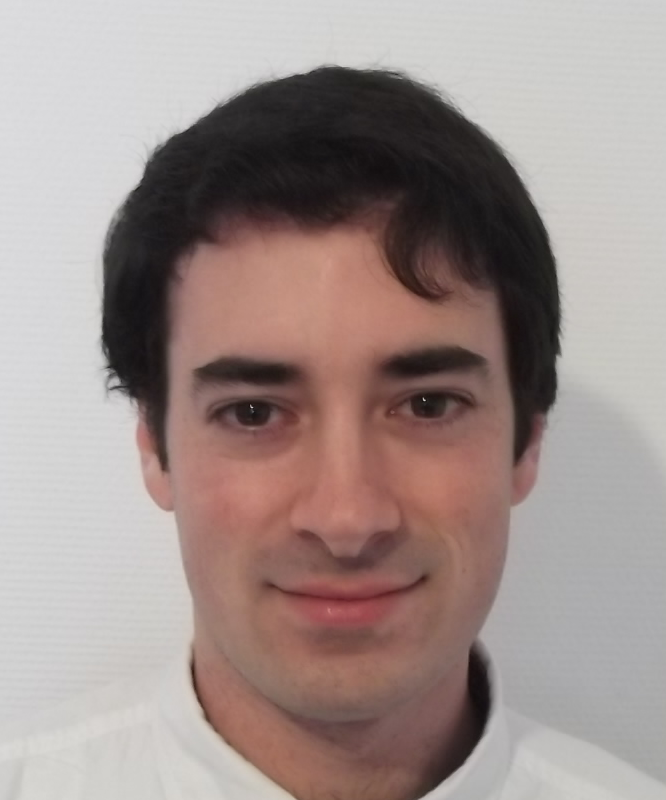
\includegraphics[width=0.18\textwidth]{photo_cv.png}
%%   \end{center}
%%   \vspace{-10pt}
%%   \vspace{-100pt}
%% \end{wrapfigure}


\begin{tabular*}{7in}{l c r}%@{\extracolsep{\fill}}r}
  \textbf{\Large Lux Benjamin}  \\ %\textbf{\today} \\
  Ingénieur en informatique  \\
  25 ans - Permis B          & \LARGE{Ingénieur en Informatique}\\ % &   \includegraphics[width=0.15\textwidth]{flower.jpg}\\
  benjamin0lux@gmail.fr      & Dans le domaine du HPC\\ 
  06\,12\,89\,07\,20           %%&  à partir d'octobre 2013\\

  %6 rue de Candale        &  à partir d'octobre 2013\\
  %33000 Bordeaux \\

\end{tabular*}





%%%\center{\huge Recherche d'un stage de deuxième année\\
%%%juin - septembre 2012}\\



%%%%%%%%%%%%%%%%%%%%%%%%%%%%%%
\resheading{Compétences}
%%%%%%%%%%%%%%%%%%%%%%%%%%%%%%
\begin{itemize}
\item[]\textbf{Compétences pratiques:}
  \begin{itemize}
  \item[]{Langages:} C, C++, C\#, Bash, Fortran, Java, Python, SQL, \LaTeX.
  \item[]{Bibliothèques pour le parallélisme:} MPI, OpenMP, threads posix, OpenCL.
    %  \item[]{Système:}
    %    Programmation système en C, multi-threads, multi-c\oe{}ur et GPU.
  \end{itemize}
\item[]\textbf{Connaissances théoriques:}
  \begin{itemize}
  \item[]{Algorithmique parallèle, calcul matriciel, algorithmique des graphes, ordonnancement.}
    
    %%   \item[]{Notions de compilation, mises en application avec Yacc et
    %%     Bison.  Notions de recherche opérationnelle, mises en application
    %%     avec Cplex.  Notions de base de données avancées, mises en
    %%     applicaton avec datalog et prolog.  ,
    %%     flots et combinatoire.  Notions de gestion de projet avec le
    %%     langage UML.}
  \end{itemize}
\item[]\textbf{Environnement de travail:}
  %\item[]{Environnement de développement:}
  \begin{itemize}
  \item[]{Environnement de développement:} Emacs, Visual Studio 2010/2008, Eclipse, Codeblocks.
  \item[]{Système d'exploitation:} Linux, Windows.% (Seven, xp).}
  \end{itemize}
  
\item[]\textbf{Langues:}
  \begin{itemize}
  \item[]{Anglais : Écrit et parlé scolaire, maîtrise du vocabulaire informatique (830 au Toeic).}
  \item[]{Espagnol : Écrit et parlé couramment.}
  \end{itemize}
\end{itemize}



%%%%%%%%%%%%%%%%%%%%%%%%%%%%%%
\resheading{Expériences}
%%%%%%%%%%%%%%%%%%%%%%%%%%%%%%

\begin{itemize}

%% \item[]
%%   \ressubheading{Inria}{Pau}{Ingénieur Jeune Diplômé}{Novembre 2014 - ...}
%%   \begin{itemize}
%%     \resitem{Développement de la bibliothèque Aerosol au sein de l'équipe CAGIRE. Implémentation de pré-conditionneurs et de méthodes multi-gilles par agrégation sur des maillages non structurés. }
%%   \end{itemize}


\item[]
  \ressubheading{Inria}{Bordeaux}{Stage de recherche}{Mars 2013 - Septembre 2013}
  \begin{itemize}
    \resitem{Optimisation de l'ordonnancement et du partitionnement d'un couplage de code de simulation de diffusion de la chaleur en parallèle (centaines de c\oe urs), en partenariat avec le CERFACS.}
    %\resitem{Optimisation de l'ordonnancement et du partitionnement du couplage des codes hautement parallèles (12000 coeurs) de simulation de diffusion de la chaleur AVTP-AVBP (CERFACS).}
  \end{itemize}


\item[]
  \ressubheading{MaxSea International}{Bidart}{Stage de développement}{Juin 2012 - Septembre 2012}
  \begin{itemize}
    \resitem{Exportation et parallélisation d'une chaine de production de cartes géographiques marines au format vectoriel dans le Cloud Microsoft Azure.}
  \end{itemize}  

\item[] 
  \ressubheading{Expérience scolaire}{Bordeaux}{Réalisation d'une interface}{2011 - 2012}
  \begin{itemize}
    \resitem{Réalisation d'une IHM et ajout de formats de sortie pour un logiciel de traduction de Braille Musical
      pour un client, enseignant-chercheur à l'Inria.}
  \end{itemize}  

%\item[]
%  \ressubheading{Travaux Saisonniers}{France, Espagne, Irlande}{Divers emplois saisonniers : \textnormal{Travaux agricoles, menuiserie, restauration.}}{étés 2006 à 2013}

\end{itemize}


%%%%%%%%%%%%%%%%%%%%%%%%%%%%%%
\resheading{Formation}
%%%%%%%%%%%%%%%%%%%%%%%%%%%%%%
\begin{itemize}
  %  \ressubheading{Enseirb-Matmeca}{Bordeaux}{ \textnormal{ Diplome d'ingénieur en informatique, option calcul parallèle.}}{2010 -- 2013}
\item[]
  \ressubheading{Enseirb-Matmeca}{Bordeaux}{ \textnormal{ Diplôme d'ingénieur en informatique, option PRCD}}{2010 -- 2013}\\
  \hspace{4ex} (Parallélisme, Régulation et Calcul Distribué). \\
\item[]
  \ressubheading{Lycée Louis Barthou}{Pau}{ \textnormal{ Élève en classes préparatoires, en Mathématiques et Physique, option informatique.}}{2007 -- 2010}  \\
\item[]
  \ressubheading{Lycée Victor Duruy}{Mont-de-Marsan}{ \textnormal{ Baccalauréat Scientifique avec mention assez bien.}}{2004 -- 2007}  \\
\end{itemize}


%% %%%%%%%%%%%%%%%%%%%%%%%%%%%%%%
\resheading{Centres d'intérêt}
%% %%%%%%%%%%%%%%%%%%%%%%%%%%%%%%
\begin{itemize}
\item[] \textbf{Loisirs :} jonglerie, lecture, jeu vidéo, vélo, kayak-polo.
\item[] \textbf{Associatif :} Membre de l'association Jonglargonne. %Membre du club de jonglage et du club Bd de l'Enseirb-Matmeca.
\end{itemize}


\end{document}
